	\chapter{Testfälle und Resultate}
	In diesem Abschnitt sollen die Ergebnisse und die Effizienz des in Abschnitt \ref{cha:program_description} vorgestellten Programmes anhand von zwei unterschiedlichen Testfällen analysiert werden. Als Referenz dient dabei das Programm \mctd \citep{Wolf:2003p12974}, sowohl für die berechneten Bilder als auch für die Geschwindigkeit der Berechnung. Für den ersten Testfall wurde zur Berechnung einer Referenzlösung zusätzlich zum einen ein geschlossener Ausdruck für die Lösung hergeleitet und zum anderen ein einfaches Monte--Carlo--Verfahren erdacht, das sehr schnell konvergiert.
	
	\section{Homogene streuende Kugel}
	Um die Korrektheit der vom Monte--Carlo--Code produzierten Lösung zu verifizieren ist es von erheblichem Nutzen eine unabhängig gewonnene, vielleicht sogar analytisch hergeleitete, Lösung eines konstruierten Testproblems berechnen zu können. Das Problem sollte dabei nicht so trivial sein, dass komplexe Effekte wie Mehrfachstreuung keinen Einfluß auf das Ergebnis haben. Gleichzeitig sollte es aber nicht so komplex sein, dass keine elegante, leicht berechenbare Lösung gefunden werden kann.
	Mit dieser Motivation konstruieren wir folgendes Testproblem:
		
	Gegeben sei eine Kugel mit Radius $R$, die mit homogenem, isotrop streuendem Material mit Volumenstreuquerschnitt $\sigma=1$ gefüllt ist, sowie eine punktförmige Lichtquelle im Zentrum der Kugel. Zu berechnen ist nun die radiale Abhängigkeit der Intensität, die eine ausserhalb der Kugel platzierte orthographische Kamera, die zum Zentrum der Kugel ausgerichtet ist, misst. Die feste Wahl von $\sigma$ und Variation des Kugelradius $R$ dient ausschliesslich der einfacheren Berechnung, da die Wegstrecken dadurch automatisch in freien optischen  Weglängen $\lambda=1/\sigma$ vorliegen. Das Problem ist gleichwertig zu jeder anderen Kombination aus Radius und Volumenstreuquerschnitt für welche sich die gleiche optische Tiefe $\tau_\text{center}=\sigma R=R/\lambda$ vom Zentrum bis zum Rand der Kugel ergibt.
	
	\begin{figure}
			\centering
			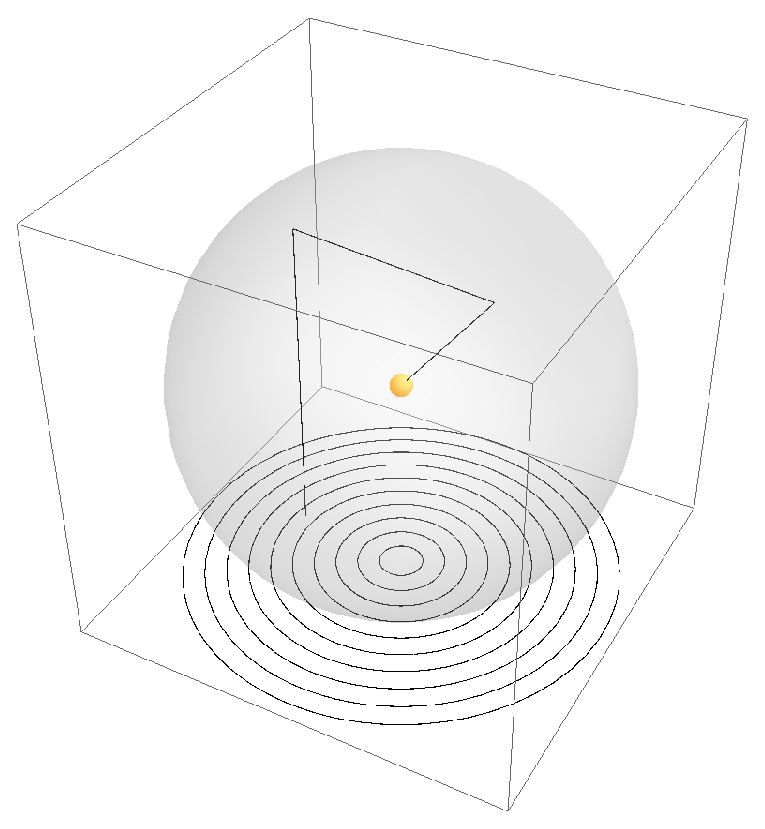
\includegraphics[height=0.3\textheight]{testproblem_illustration.eps}
			\caption{Illustration des Testproblems. Gezeigt ist ein Photonenpfad der zweimal gestreut wird und in einem ringförmigen Bin der orthographischen Kamera auftrifft}
			\label{fig:testproblem_sketch}
	\end{figure}

	
	\subsection{analytische Lösung}\label{subsec:homsphere_analytic_solution}
	\subsubsection{Green'sche Funktion für den Photonentransport zwischen Kugelschalen}
	Um die korrekte radiale Intensitätsverteilung zu berechnen, bestimmen wir zunächst in Form der Green'schen Funktion $g$, wie sich die Photonen radial nach einem Streuvorgang ausgebreitet haben.
	Genauer gibt $g$ an, wie groß der Anteil der Photonen, die auf einer Kugelschale mit Radius $r_0$ starten, beim Radius $r_1$ während des nächsten Streuvorganges ist (siehe Abb. \ref{fig:radial_greens_function_pdfcdf}):
	\begin{align*}
		g(r_0,r_1) =& 2 \pi \int_0^\pi r_1^2 \sin(\theta) \frac{\exp\left(-\sqrt{r_0^2-2 r_0 r_1 \cos(\theta)+r_1^2}\right)}{4 \pi (r_0^2-2 r_0 r_1 \cos(\theta)+r_1^2)} \text{d}\theta \\
		=& \frac{1}{2}\frac{r_1}{r_0} \int_{|r_0-r_1|}^{r_0+r_1} \frac{e^{-t}}{t} dt \\
		=& \frac{1}{2}\frac{r_1}{r_0}\left[\text{Ei}(-(r_0+r_1)) - \text{Ei}(-|r_0-r_1|)\right]
	\end{align*}
	
	\begin{figure}
		\centering
		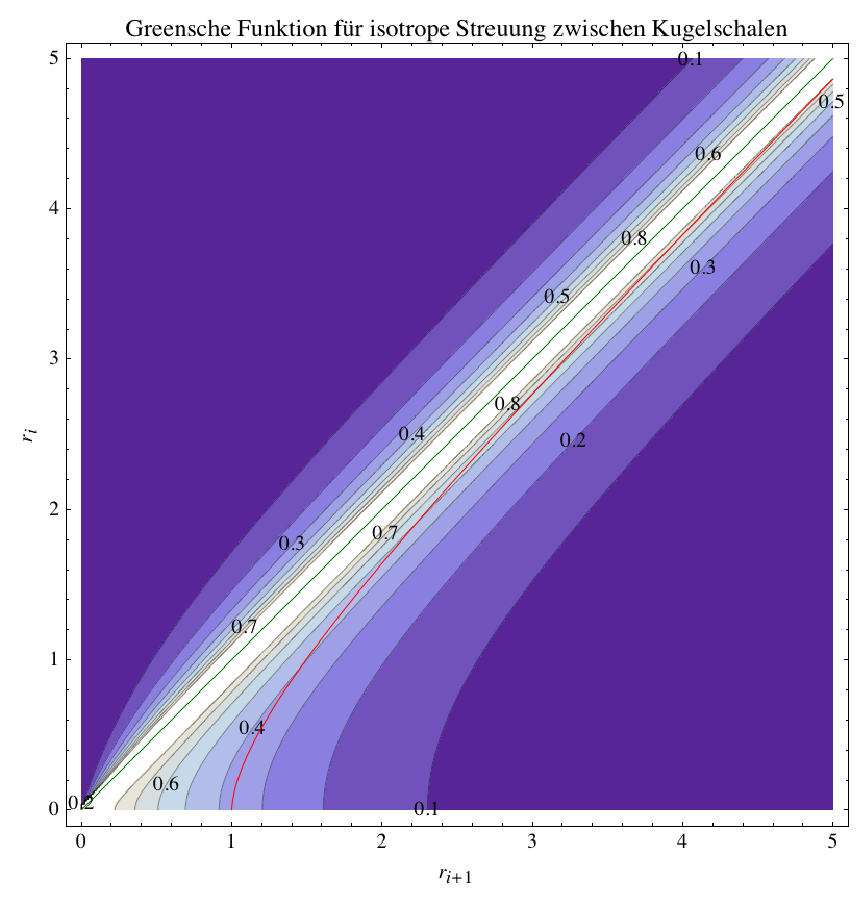
\includegraphics[width=0.48\textwidth]{radial_greens_function_pdf.eps}
		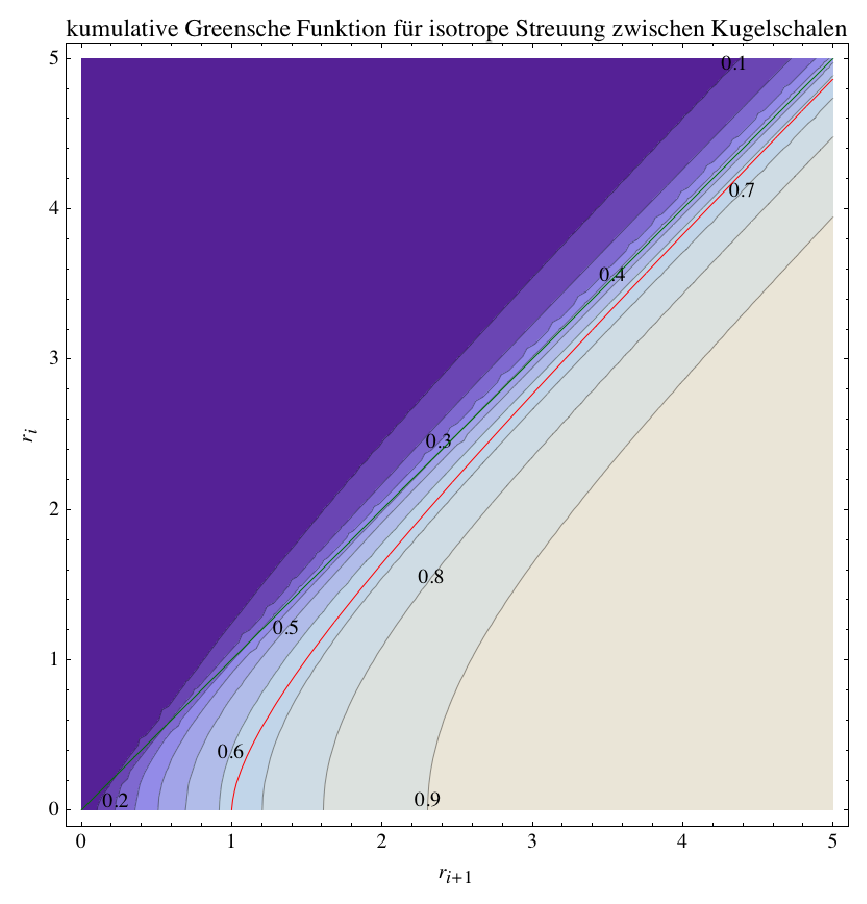
\includegraphics[width=0.48\textwidth]{radial_greens_function_cdf.eps}
		\caption{Green'sche Funktion der radialen Teilchenverteilung die von Radius $r_i$ kommen und beim Radius $r_{i+1}$ streuen als PDF und CDF. Der mittlere Radius ist in rot eingezeichnet.}
		\label{fig:radial_greens_function_pdfcdf}
	\end{figure}
	\begin{figure}
		\centering
		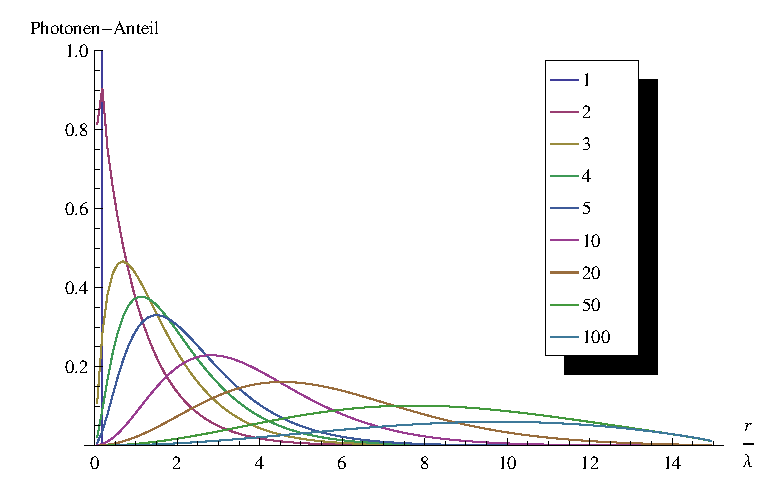
\includegraphics[width=0.9\textwidth]{gnlist_plot.eps}
		\caption{radiale Photonenverteilung nach n Streuvorgängen. Die freie optische Weglänge ist dabei mit $\lambda=1/\sigma$ bezeichnet.}
		\label{fig:gnlist}
	\end{figure}
	Als nächstes diskretisieren wir die Green'sche Funktion, indem wir ein gleichmäßiges Gitter in $r_0$ und $r_1$ über $g$ legen, das sich bis zum Radius der Kugel $R$ erstreckt, und innerhalb jeder Gitterzelle $g$ in $r_0$--Richtung mitteln und in $r_1$--Richtung aufintegrieren und anschliessend die Ergebnisse in einer Matrix $\mathbf{g}$ speichern. Wenn wir nun einen Startvektor, der nur in der innersten Zelle von Null verschieden ist, $n$--mal mit $\mathbf{g}$ multiplizieren, bekommen wir die diskretisierte Photonenverteilung innerhalb der Kugelschalen beim $n$--ten Streuvorgang (siehe Abb. \ref{fig:gnlist}). Um die Emissivität $\varepsilon(r)$ jeder Kugelschale auszurechnen, summieren wir die Photonenverteilungen vom 1--ten bis zum $n$--ten Streuvorgang auf und teilen das Ergebnis in jeder Kugelschale durch ihr jeweiliges Volumen und den bestrahlten Raumwinkel $4\pi$. Die Intensitäten können nun numerisch gemäß
	\begin{equation}
		I(r) = \int_{z=-h}^h \varepsilon\left(\sqrt{r^2+z^2}\right) e^{-(z+h)}\text{d}z\,,\quad h=\sqrt{R^2-r^2}
		\label{eq:testprob_intensity_calculation}
	\end{equation}
	berechnet werden.
	
	%\begin{figure}
	%	\centering
	%	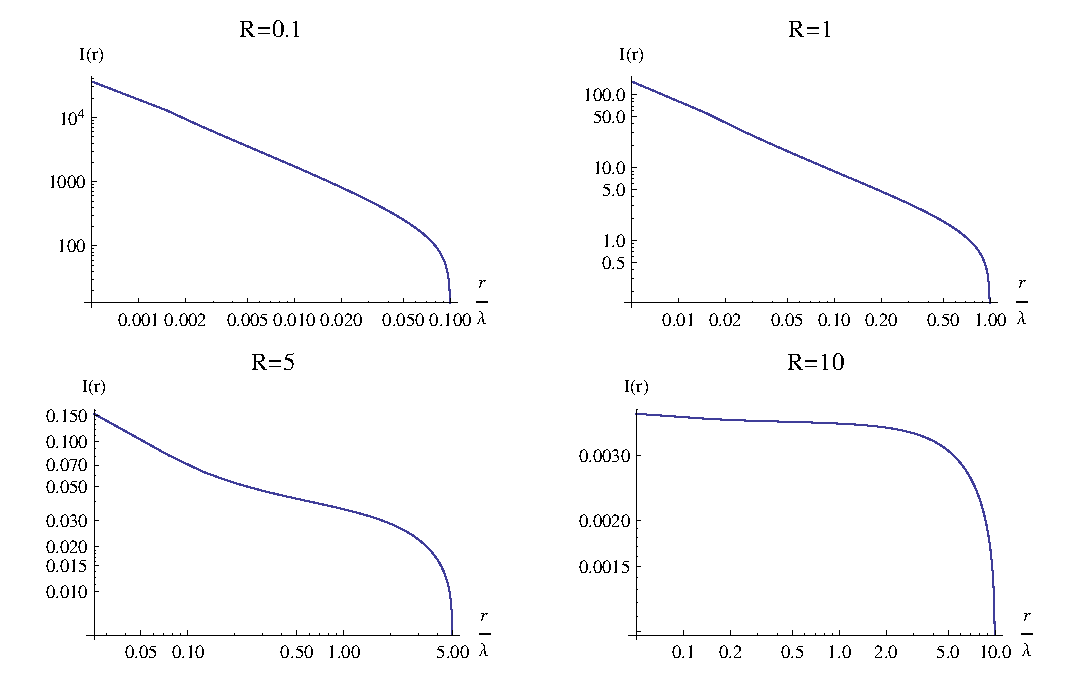
\includegraphics[width=1.0\textwidth]{analytical_tau_comparison.eps}
	%	\caption{radiales Intensitätsprofil für verschiedene Kugelradien und damit verschiedene optische Tiefen. $\lambda=1/\sigma$ bezeichnet die freie optische Weglänge.}
	%	\label{fig:analytical_tau_comparison}
	%\end{figure}
	
	%Das Ergebnis ist für vier Kugelradien beispielhaft in Abb. \ref{fig:analytical_tau_comparison} dargestellt.
	
	\vfill
	\pagebreak
	\subsection{schnelle Monte--Carlo--Lösung}
	Eine andere Methode, schnell die radiale Intensitätsverteilung zu bestimmen, ist durch folgendes Monte--Carlo--Schema gegeben:
	\begin{algorithmic}
		\STATE $M\leftarrow$ Anzahl Ringe
		\STATE $N\leftarrow$ Anzahl Photonen
		\STATE $R\leftarrow$ Kugelradius
		\FOR{$i=1$ to $N$}
			\STATE $\location{r}\leftarrow (0,0,0)^\text{T}$
			\REPEAT
				\STATE\COMMENT{wähle zufällige Richtung $\omega$}
				\STATE $z\leftarrow$ ziehe gleichförmig aus $[-1,1]$
				\STATE $\phi\leftarrow$ ziehe gleichförmig aus $[0,2\pi]$
				\STATE $s\leftarrow\sqrt{1-z^2}$
				\STATE $\omega\leftarrow (s\;\text{cos}(\phi),s\;\text{sin}(\phi),z)^\text{T}$
				\STATE\COMMENT{wähle exponentiell verteilte Entfernung $t$}
				\STATE $u\leftarrow$ ziehe gleichförmig aus $[0,1]$
				\STATE $t\leftarrow -\text{ln}(1-u)$
				\STATE $\location{r}_\text{old}\leftarrow\location{r}$
				\STATE $\location{r}\leftarrow\location{r}_\text{old}+\omega t$
			\UNTIL{$|\location{r}|\geq R$}
			\STATE\COMMENT{bestimme Stoßparameter $b$}
			\STATE $\location{d}\leftarrow\location{r}-\location{r}_\text{old}$
			\STATE $b\leftarrow\sqrt{\langle\location{r},\location{r}\rangle-\frac{\langle\location{r},\location{d}\rangle}{\langle\location{d},\location{d}\rangle}}$
			\STATE $j\leftarrow\lfloor M\frac{b}{R}\rfloor$
			\STATE $C[j]=C[j]+1$
		\ENDFOR
		\FOR[normiere Bincounts mit Ringflächen]{$j=0$ to $M-1$}
			\STATE $C[j]=C[j]/(\pi R^2(2j+1)/M^2)$
		\ENDFOR
		\RETURN $C[\cdots]$
	\end{algorithmic}
	Dabei starten wir mit einem Photon im Ursprung und berechnen dann von der aktuellen Position solange die Position des nächsten Streuereignisses, bis dieses ausserhalb der Kugel liegt. Damit kennen wir den letzten Streupunkt und die Richtung in die das Photon das Streuvolumen verlässt. Da wir nur an der radialen Intensitätsverteilung interessiert sind können wir die Symmetrie des Problems ausnutzen indem wir die Kamera immer so hindrehen, dass das entfliehende Photon senkrecht auf den (gedachten) Sensor auftrifft. Das bedeutet, dass nicht die genaue Entweichrichtung sondern nur der Stoßparameter entscheidend ist. Mit diesem Trick können wir jedes entweichende Photon zählen, sodass dieses Verfahren sehr schnell konvergiert.
	
	
	\subsection{Resultate}
	Um die korrekte Berechnung des Strahlungstransports überprüfen zu können, simulieren wir das vorgestellte Problem der homogen streuenden Kugel für drei verschiedene Radien (und damit optische Tiefen) jeweils mit der in Abschnitt~\ref{subsec:homsphere_analytic_solution} vorgestellten Methode, die wir als Referenzlösung benutzen. Dieselben Konfigurationen berechnen wir außerdem mit \mctd und \pirate. Von \mctd lassen wir hierfür $3.6\cdot10^8$ Photonen generieren und von 72 virtuellen Kameras, die auf einem Kreis auf das Zentrum blickend im Abstand von 5 Grad verteilt sind, beobachten. Jede Kamera ist dabei in einem Kegel mit öffnungswinkel von $\alpha=5^\circ$ für eintreffende Photonen empfindlich\footnote{In Abb.~\ref{fig:alphacomparison} ist der Effekt unterschiedlicher Kameraöffnungswinkel $\alpha$ bei gleicher Photonenanzahl gezeigt.}. \pirate benutzt eine einzige Kamera deren Empfindlichkeitskegel einen öffnungswinkel von $30'$ besitzt. Hier generieren wir die Bilder in mehreren unabhängigen Läufen mit Pfadanzahlen zwischen $10^5$ und $10^7$.
	
		\begin{figure}
			\centering
			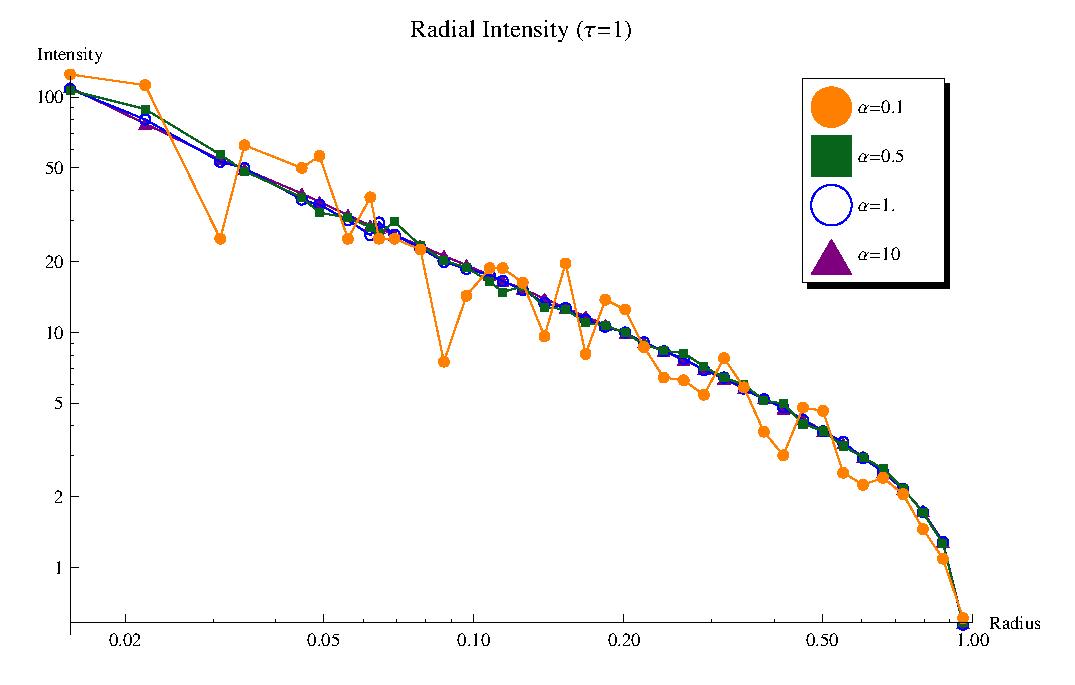
\includegraphics[width=0.8\textwidth]{mc3dalphasplot.eps}
			\caption{Radiale Intensitätsprofile auf der Grundlage von \mctd--Simulationen --- Bei gleicher Photonenzahl aber sinkendem Kamera--öffnungswinkel $\alpha$ steigt der statistische Fehler aufgrund der geringeren Zahl beachteter Photonen.}
			\label{fig:alphacomparison}
		\end{figure}
		
	Die drei zur Simulation gewählten optischen Tiefen $\tau\in\{0.01,1,10\}$ decken den optisch dünnen, mittleren und dicken Fall ab.	In Abb.~\ref{fig:methodcomparisongraphics} sind mit der analytischen Methode, \mctd und \pirate gewonnene radiale Intensitätsprofile abgebildet.
	Im dargestellten Bereich stimmen die Ergebnisse beider Programme im Rahmen des statistischen Fehlers gut mit der analytischen Lösung überein. Dabei ist zu bedenken, dass bei kleineren Radien über weniger Pixel der zugrundeliegenden Bilder gemittelt wird und somit der statistische Fehler dort naturgemäß größer ausfällt.
		\begin{figure}
			\centering
			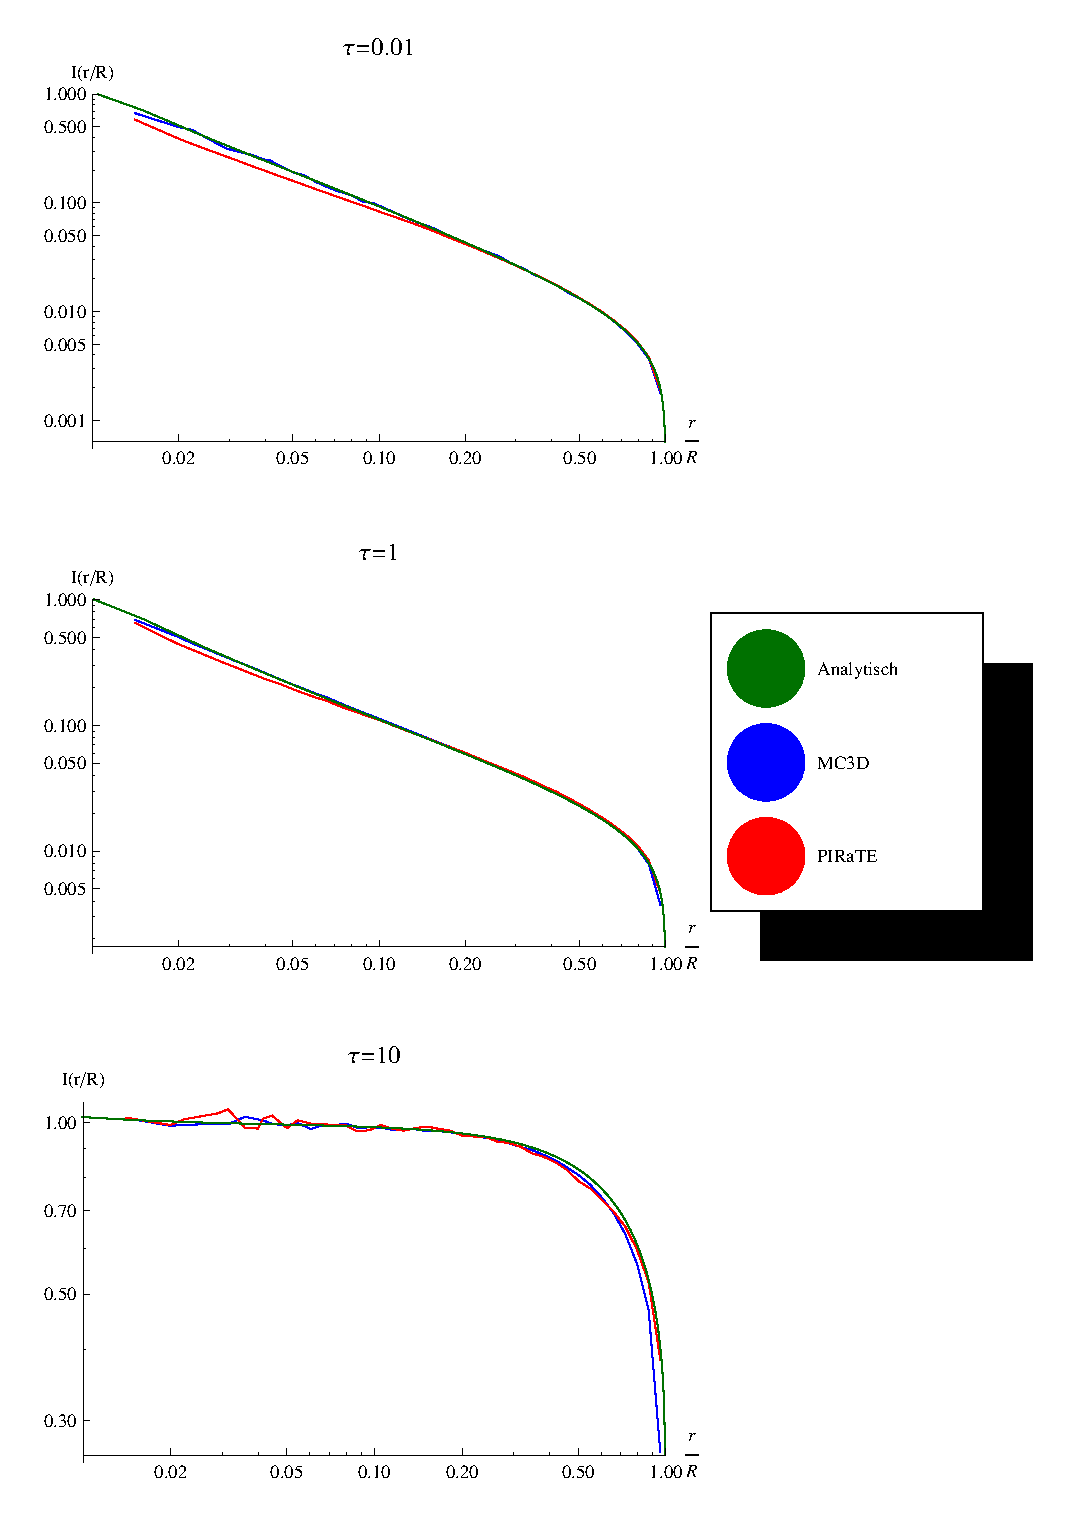
\includegraphics[height=1.0\textheight]{methodcomparisongraphics.eps}
			\caption{Vergleich zwischen der analytischen Lösung, \mctd und \pirate bei verschiedenen optischen Tiefen. \mctd hat für alle drei Fälle $3.6\cdot10^8$ Photonen, \pirate jeweils $4.88\cdot10^7,4.88\cdot10^7,2.088\cdot10^8$ Photonenpfade generiert.}
			\label{fig:methodcomparisongraphics}
		\end{figure}
	
	Bei Betrachtung von horizontalen Schnitten durch die Streubilder (siehe Abb.~\ref{fig:sphere_image_cuts}) fällt auf, das \pirate den Anteil des direkt von der Punktlichtquelle kommenden Lichtes falsch schätzt. Dies liegt vermutlich an den Sensorparametern (insbesondere dem öffnungswinkel), da im Unterschied zu \mctd in \pirate keine punktförmigen sondern nur ausgedehnte Lichtquellen existieren, die bei kleinen Ausmaßen mit der jetzigen Pfadgenerierungsmethode schwer zu samplen sein können. Zur endültigen Klärung bedarf es aber einer genaueren Fehleranalyse.
	
		\begin{figure}
			\centering
			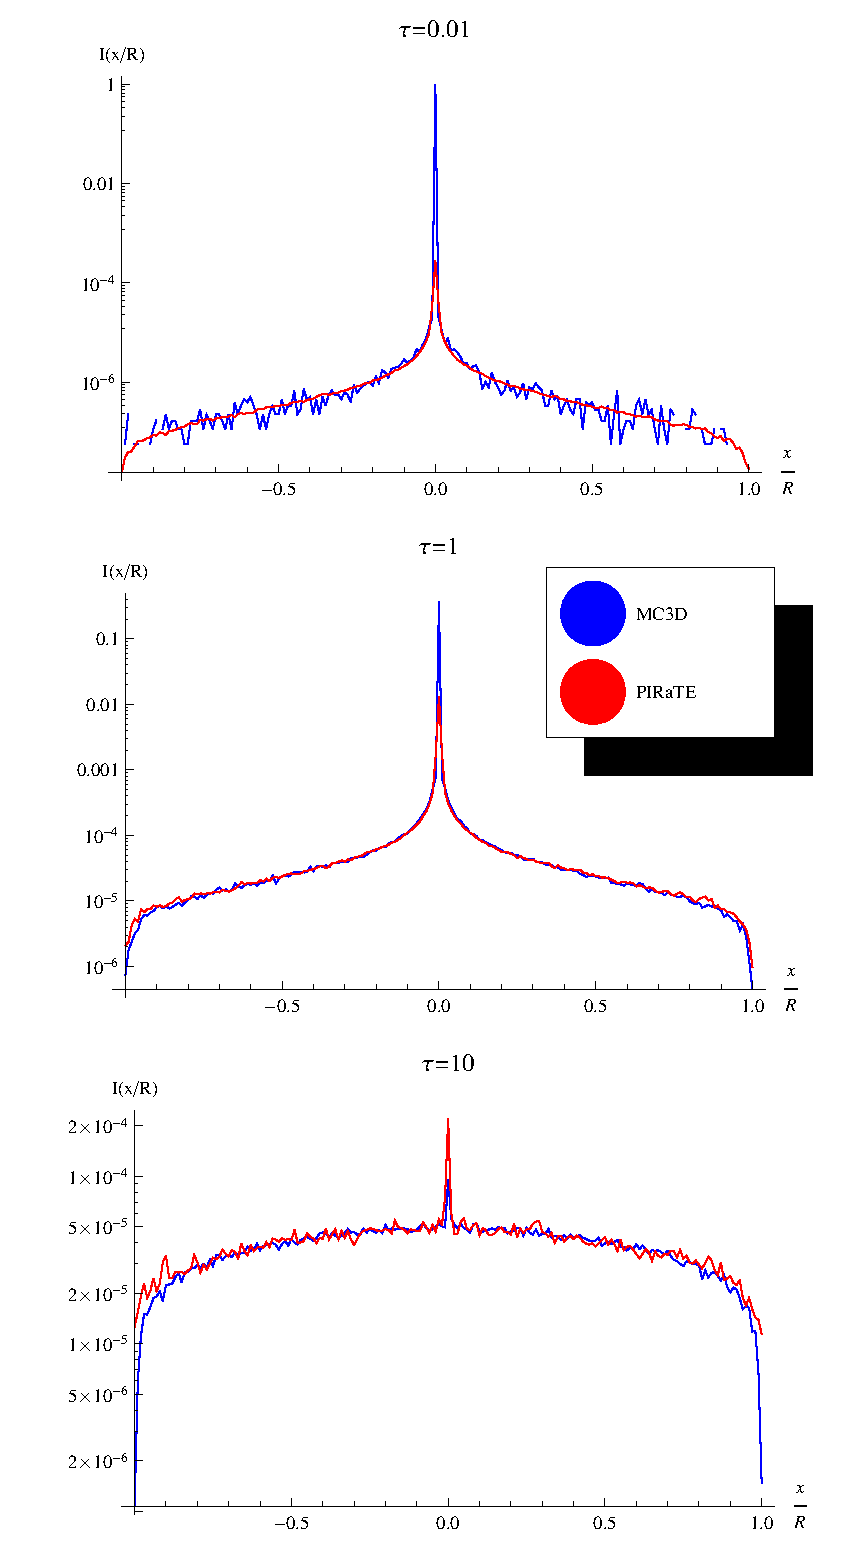
\includegraphics[height=1.0\textheight]{sphere_image_cuts.eps}
			\caption{Horizontale Schnitte durch die Streubilder für die drei optischen Tiefen bei hoher Anzahl an Photonen bzw. Pfade.}
			\label{fig:sphere_image_cuts}
		\end{figure}
	
	Um nicht komplett auf einen Vergleich der Konvergenzraten beider Programme verzichten zu müssen, verwenden wir zur Berechnung der Abweichung vom Referenzbild maskierte Bilder, bei denen die Lichtquelle in der Mitte des Bildes ausgeblendet ist.	 Die Referenzbilder %(siehe Abb.~\ref{fig:sphere_reference_images}) 
	werden dabei aus den, aus allen 72 Kameraebenen akkumulierten, von \mctd erzeugten Streubildern generiert. Zusätzlich mitteln wir innerhalb des Bildes über alle Pixelgruppen mit exakt gleichem Abstand vom Zentrum% (siehe Abb.~\ref{fig:polaraveragingsymmetry})
	. Dies führt im Durchschnitt zu einer Mittelung über 11 Pixel wodurch das Rauschen ungefähr gedrittelt wird, was insbesondere bei dem Bild der optisch dünnen Kugel, welches das stärkste Rauschen besitzt, hilfreich ist.
	
		%\begin{figure}
		%	\centering
		%	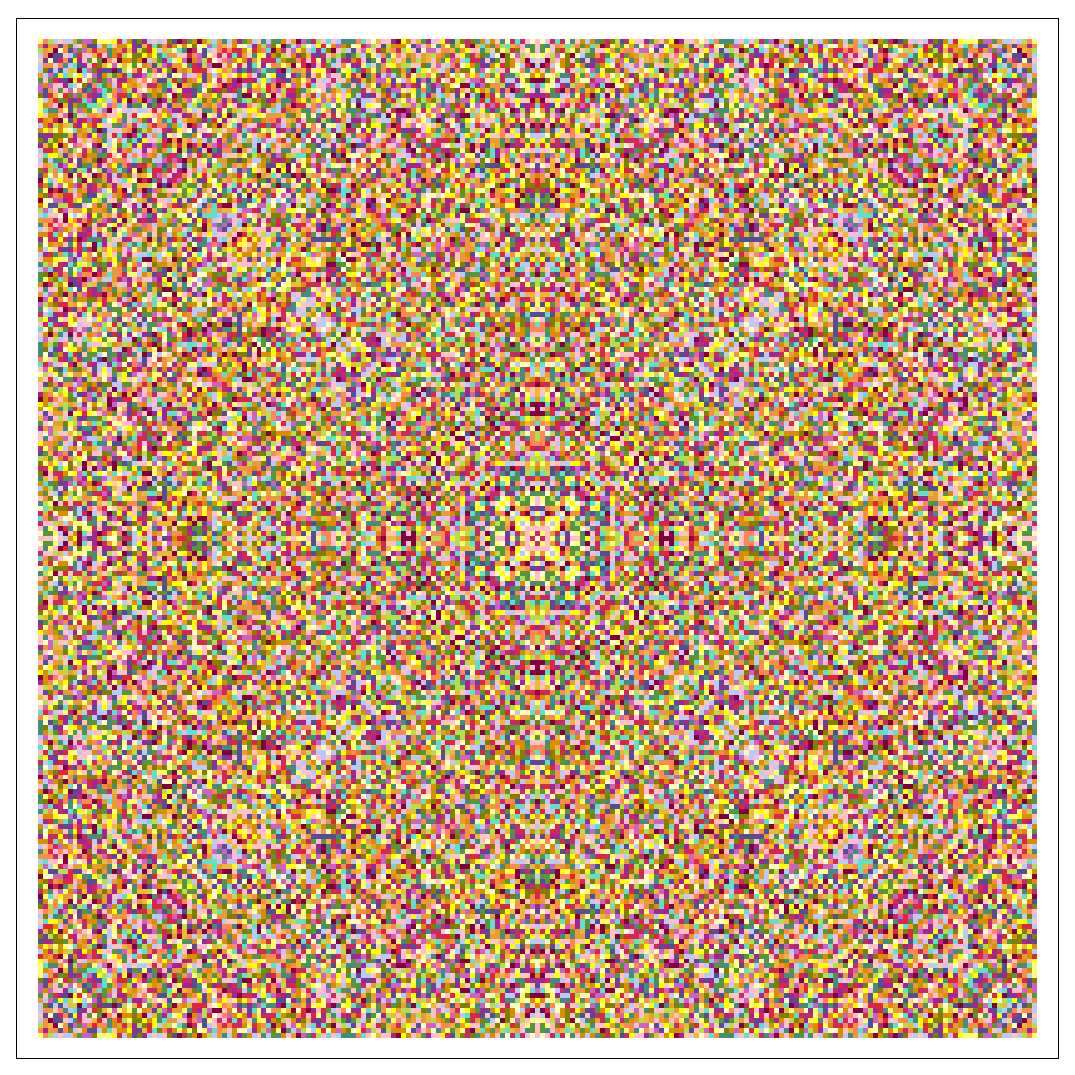
\includegraphics[width=0.5\textwidth]{polaraveragingsymmetry.eps}
		%	\caption{Darstellung der Symmetrien, die bei der polaren Mittelung genutzt werden. Pixel mit exakt gleichem Abstand zum Zentrum sind gleich gefärbt. Im Schnitt wird über 11 Pixel gemittelt.}
		%	\label{fig:polaraveragingsymmetry}
		%\end{figure}
		
		%\begin{figure}
		%	\centering
		%	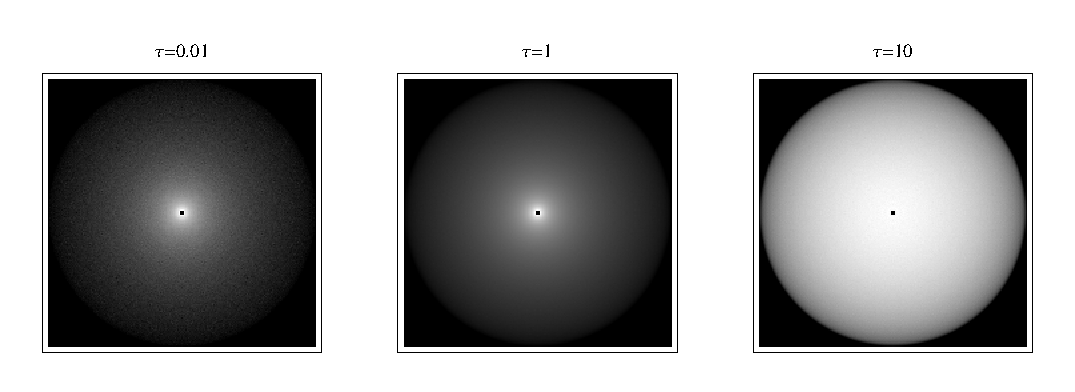
\includegraphics[width=1.0\textwidth]{spherereferenceimages.eps}
		%	\caption{Referenzbilder zur Bestimmung der Abweichungen}
		%	\label{fig:sphere_reference_images}
		%\end{figure}
	
	Eine Auswahl der generierten Streubilder ist in den Abbildungen \ref{fig:mc3d_sphere_imageoverview} und \ref{fig:pirate_sphere_imageoverview} dargestellt und jeweils mit der Anzahl an generierten Photonen bzw. Pfaden sowie der zum generieren benötigten Rechenzeit versehen. Die \mctd--Rechenzeiten sind trotz unterschiedlicher Photonenzahlen konstant. Dies liegt daran, dass die Bilder nur unterschiedlich viele aufsummierte Kameraebenen desselben Simulationslaufes darstellen und nicht die Summe der Ergebnisse verschiedener Simulationen.
	
	Aufgrund der unterschiedlichen zugrundeliegenden Algorithmen, Programmiersprachen, Compiler und Computer mit denen die Ergebnisse erzeugt wurden, ist es schwierig die beiden Programme objektiv zu vergleichen. Während \mctd eine feste Zahl von Photonen simuliert, die entweder in einer Kameraebene aufgefangen und gezählt werden oder nicht, generiert \pirate eine feste Zahl Pfade, die den Sensor erreicht haben aber unterschiedlich stark gewichtet in das Ergebnis eingehen. Während \mctd immer von einer inhomogenen Dichteverteilung ausgeht und aufintegriert, um optische Tiefen zu bestimmen, kann \pirate die optischen Tiefen im homogenen Fall direkt berechnen. \mctd generierte die Ergebnisse auf einem Intel Xeon E5405 (2000 MHz) Prozessor--Kern, \pirate auf einem AMD Opteron 8354 (2200 MHz) Prozessor--Kern. Daher sollten die Ergebnisse als Grössenordnungsabschätzungen und nicht als absolut unumstößliche Messergebnisse interpretiert werden.
	
		\begin{figure}
			\centering
			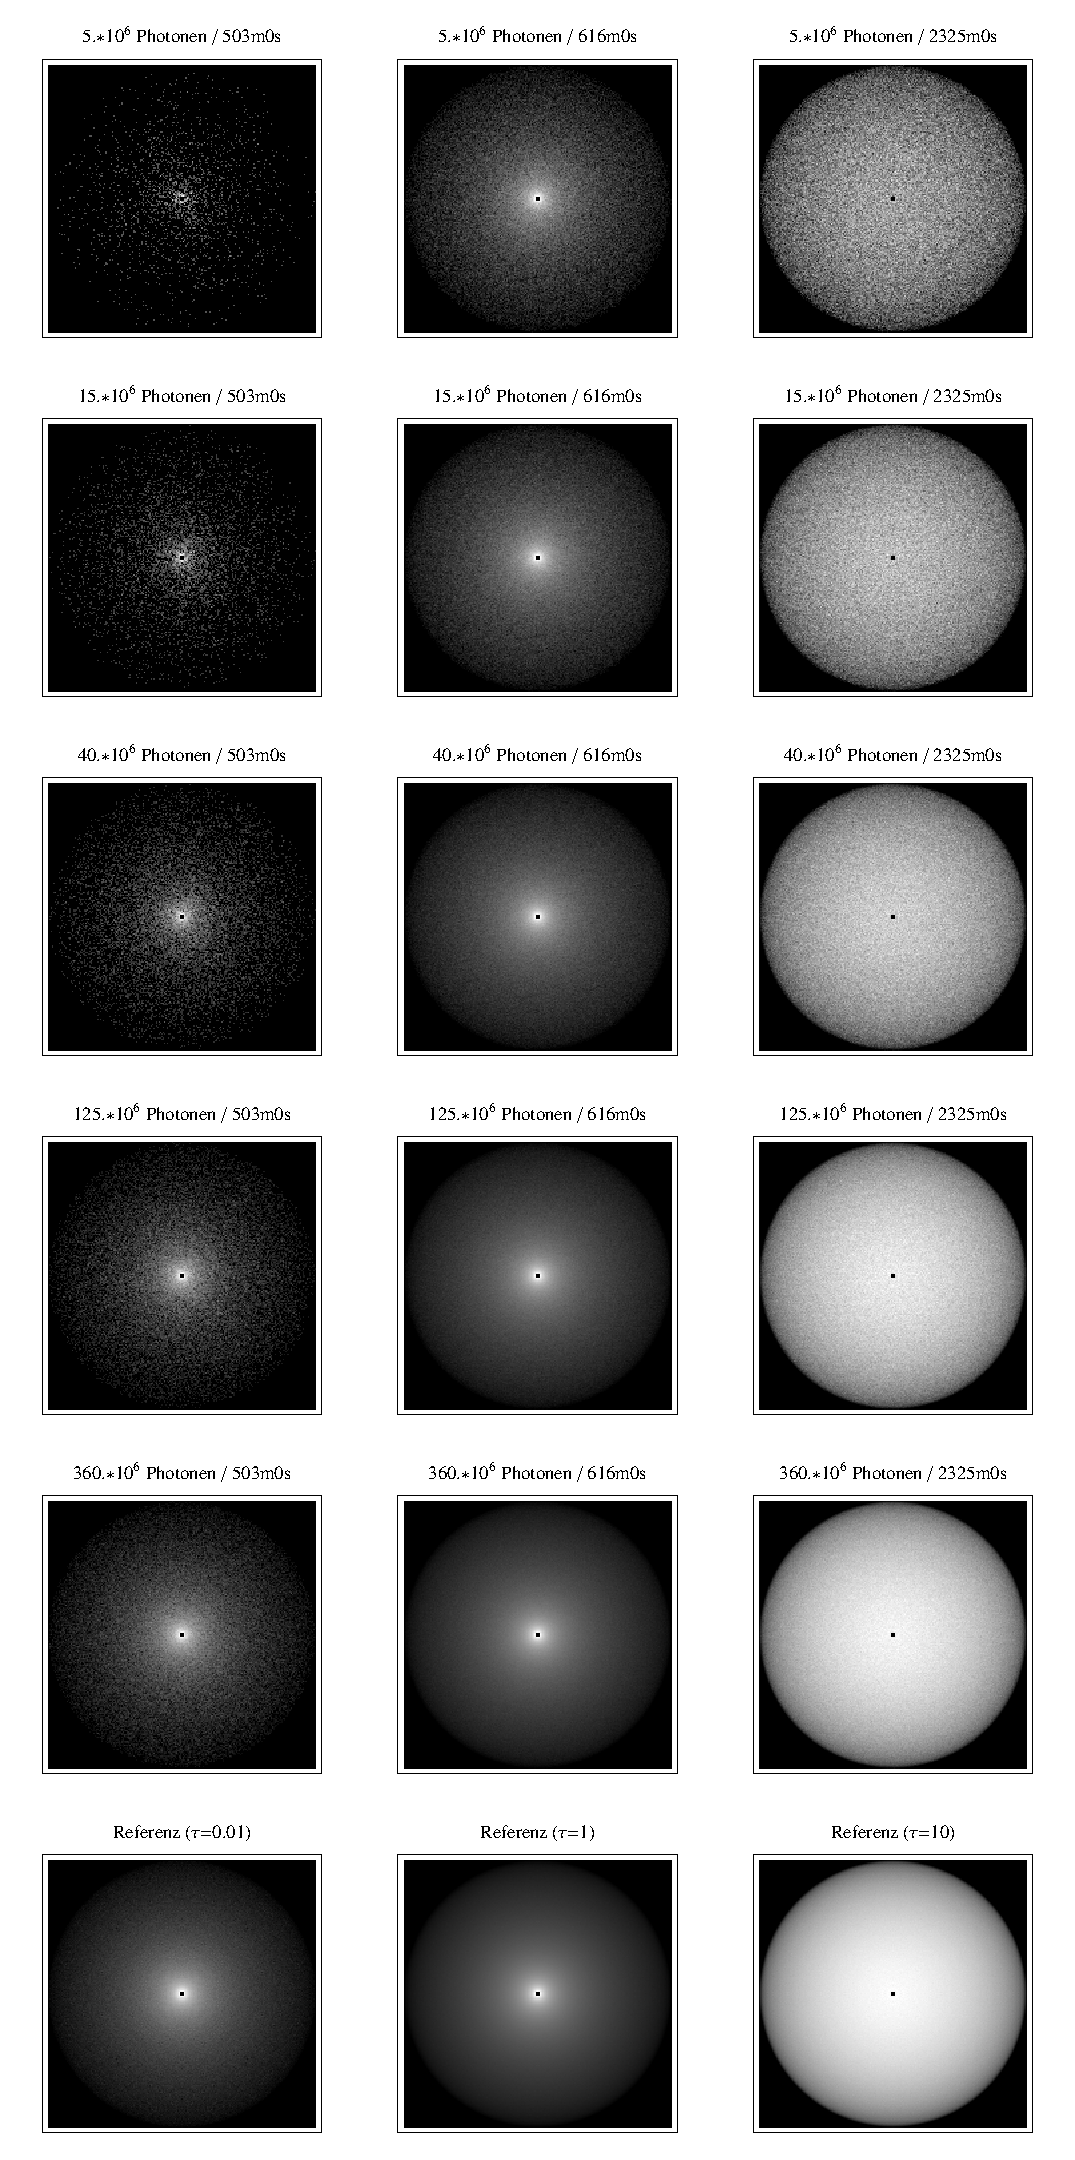
\includegraphics[height=1.0\textheight]{mc3dsphereimageoverview.eps}
			\caption{übersicht über die Qualität und Simulationszeiten der Bilder bei Akkumulation unterschiedlich vieler Kameraebenen der \mctd--Simulationen.}
			\label{fig:mc3d_sphere_imageoverview}
		\end{figure}
		\begin{figure}
			\centering
			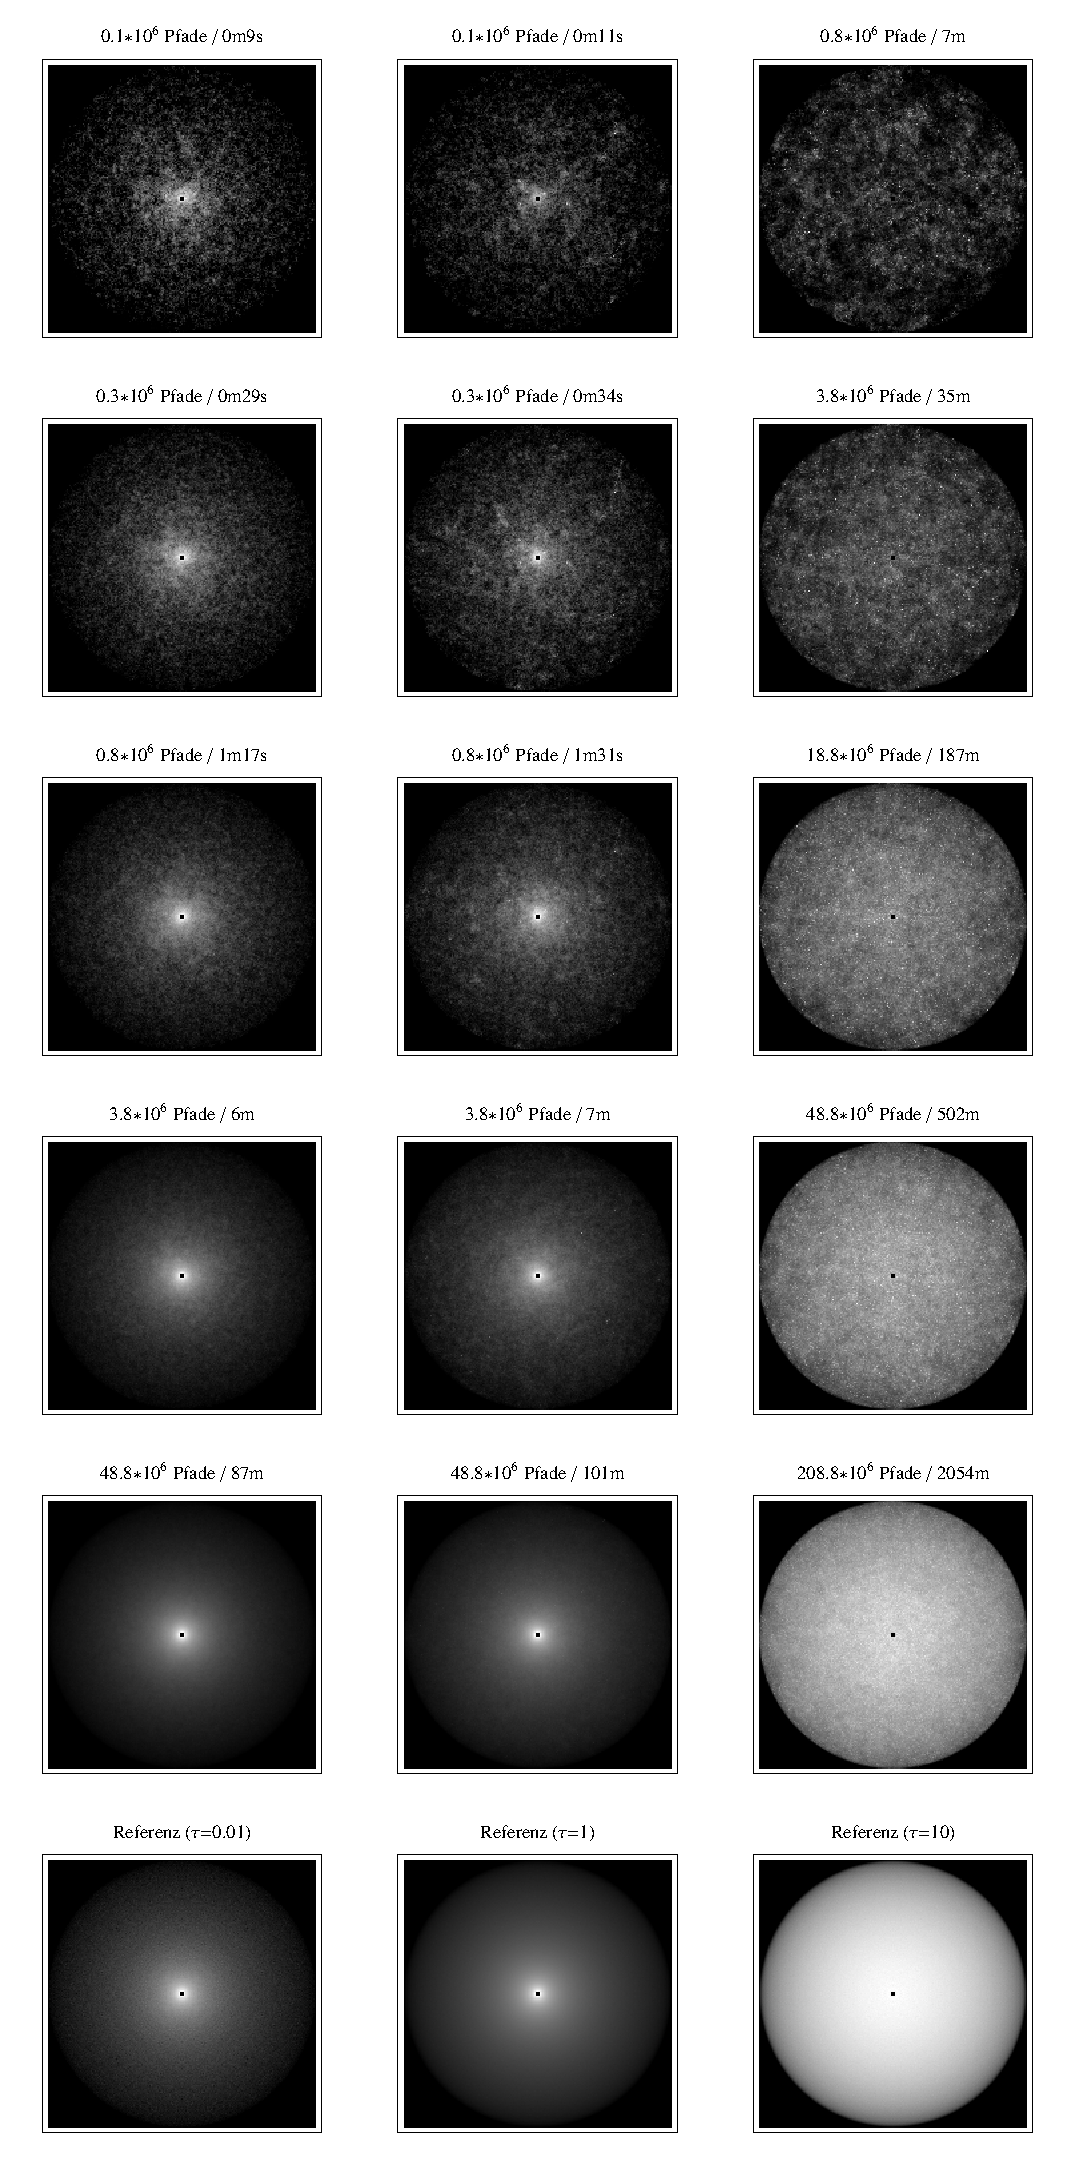
\includegraphics[height=1.0\textheight]{piratesphereimageoverview.eps}
			\caption{übersicht über die Qualität der Bilder bei unterschiedlich langen \pirate--Simulationsläufen.}
			\label{fig:pirate_sphere_imageoverview}
		\end{figure}
	
	
	In Abb.~\ref{fig:sphere_errors} ist für die verschiedenen optischen Tiefen der absolute Fehler zum Referenzbild gegen die Anzahl berechneter Photonen/Pfade bzw. die Rechenzeit aufgetragen. Der absolute Fehler wird als mittlerer quadratischer Fehler aller Pixel berechnet. Da bei \mctd die verschiedenen Streubilder nicht durch mehrere Simulationsläufe sondern mehrere Kameraebenen erzeugt wurden, sind für \mctd zwei Kurven eingezeichnet. Beide Kurven fassen die Summation unterschiedlich vieler Kameraebenen der durchgeführten Simulation als die Ergebnisse verschiedener Simulationen mit unterschiedlicher Anzahl generierter Photonen aber konstanter Kameraebenenanzahl auf. Die linke Kurve interpretiert sie als die Ergebnisse einer Simulation mit 72, die rechte als Ergebnis einer Simulation mit nur einer Kameraebenen auf.
	
	In Bezug auf die Rechenzeit ist \pirate in allen drei optischen Tiefen gleichwertig oder (besonders im optisch dünnen Fall) um mehrere Größenordnungen schneller. Dabei muß aber auch berücksichtigt werden, dass \pirate den homogenen Fall speziell behandelt und dadurch effizienter berechnen kann, wohingegen \mctd immer von inhomogenen Dichteverteilungen ausgeht.
	
	Im optisch dünnen Fall ($\tau=0.01$) erzeugt \pirate mit einer Größenordnung weniger Pfaden Bilder gleichen Fehlers. Bei nur einer Kameraebene sind es sogar drei Größenordnungen. Die Abflachung der Konvergenzrate von \pirate liegt daran, dass dort der Fehler der Simulationen unter den Rauschpegel der Referenzbilder fällt. Zur höheren Effizienz trägt vermutlich zum Großteil der verwendete Distanzsampler (siehe Gleichung \ref{eq:enforced_scattering_distancesampler}) bei, der eine mögliche Streuung erzwingt.
	
	Bei einer optischer Tiefe von $\tau=1$ liegt die Effizienz von \pirate bezogen auf die Anzahl generierter Pfade zwischen der Effizienz von \mctd mit 72 Kameraebenen und \mctd mit nur einer Kameraebene.
	
	Im Falle einer optischen Tiefe von $\tau=10$ ist die Generierung von Streubildern gleichen mittleren quadratischen Fehlers bezogen auf die Anzahl generierter Pfade mit \pirate ungefähr in der gleichen Größenordnung wie mit \mctd mit nur einer Kameraebene. Es zeigt sich also, dass die aktuell in \pirate implementierte Methode zur Pfadgenerierung bis zu dieser optischen Tiefe gut einsetzbar ist, aber für noch größere optische Tiefen in dieser Form nicht gut geeignet ist.

		\begin{figure}
			\centering
			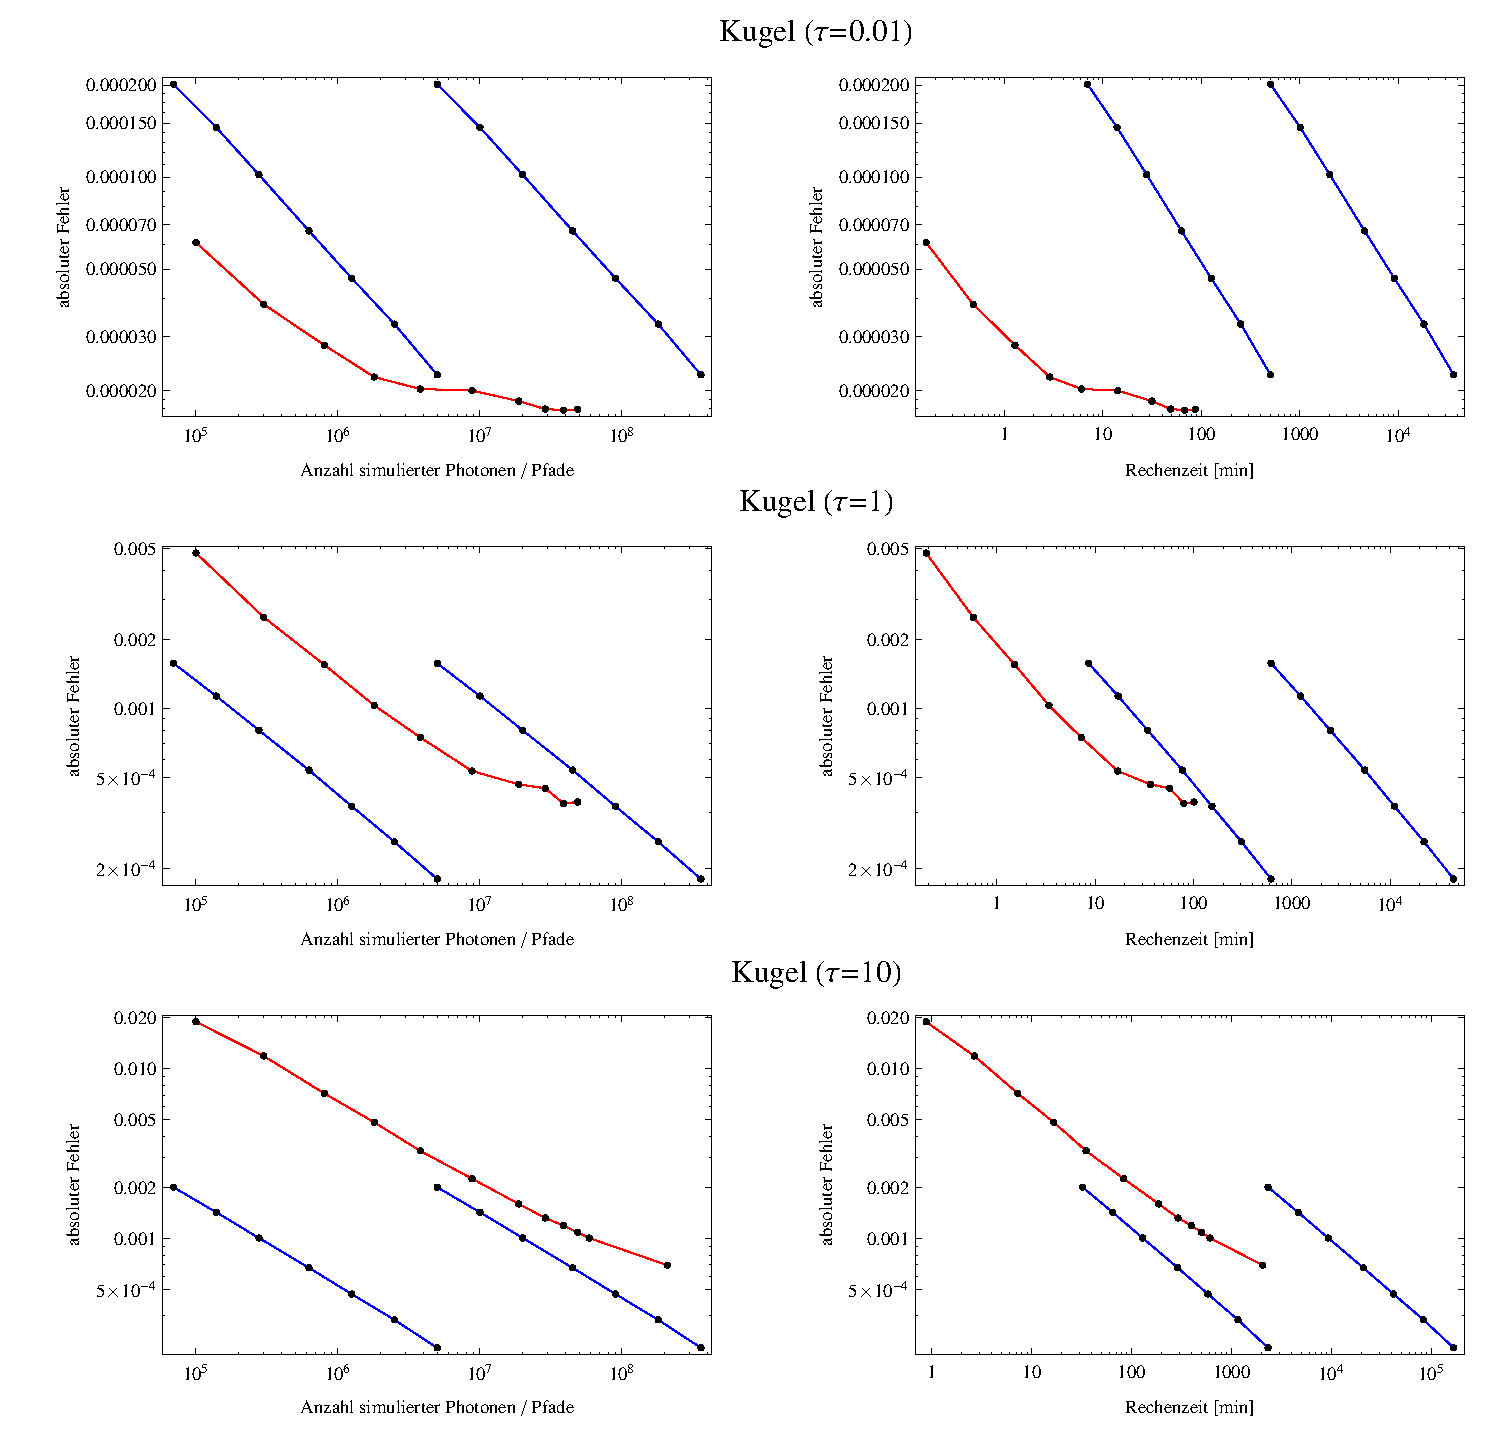
\includegraphics[width=1.0\textwidth]{sphereerrorplots.eps}
			\caption{Die rote Linie repräsentiert \pirate--Simulationen. Die blauen Linien repräsentieren \mctd. Die linke Linie steht für Simulationen mit 72, die rechte für Simulationen mit einer Kameraebene.}
			\label{fig:sphere_errors}
		\end{figure}


	\section{Einfaches Scheibenmodell}
	Als zweiten Testfall benutzen wir eine inhomogene Verteilung mit einer Scheibenstruktur mit Gauss'schem Vertikalprofil und linear steigender Skalenhöhe, die durch die Dichteverteilung (in zylindrischen Koordinaten $(s,\phi,z)$ und mit dem radialen Abstand $r=\sqrt{s^2+z^2}$)
	\begin{align}
		\rho(s,z)&=\Sigma(r)\text{exp}\left[-\frac{1}{2}\left(\frac{z}{\epsilon\,s}\right)^2\right],\quad s_\text{in}<s<s_\text{out}\land r<r_\text{out} \nonumber\\
		\Sigma(r)&=\Sigma_0 / (a^2+s^2) \label{eq:disk_model} \\
		s_\text{in}&=0.01, s_\text{out}=1, r_\text{out}=1, a=0.25, \epsilon=0.1 \nonumber
	\end{align}
	gegeben ist (siehe Abb.~\ref{fig:diskdensity}).	Dabei wählen wir $\Sigma_0$ so, daß die optische Tiefe in der Mittelebene vom Zentrum bis zum Rand der Scheibe $\tau=97.7$ beträgt. Als Materialeigenschaften nehmen wir idealisierend wieder isotrop streuendes Material mit einer Albedo von eins an.
	
		\begin{figure}
			\centering
			\includegraphics[height=0.25\textheight]{diskdensity.eps}
			\caption{Verteilung des Volumenstreuquerschnittes im Schnitt durch die x--z--Ebene der Scheibe.}
			\label{fig:diskdensity}
		\end{figure}
	
	\subsection{Resultate}
		Nach Durchführung von Simulationen mit $10^5$--$3\cdot 10^7$ Pfaden in \pirate und einer Simulation mit $7.2\cdot 10^8$ Photonen und 72 Kameraebenen in \mctd mit der Dichteverteilung (\ref{eq:disk_model}) erhalten wir die in Abb.~\ref{fig:disk_image_overview} gezeigten (und weitere) Streubilder.
		
		\begin{figure}
			\centering
			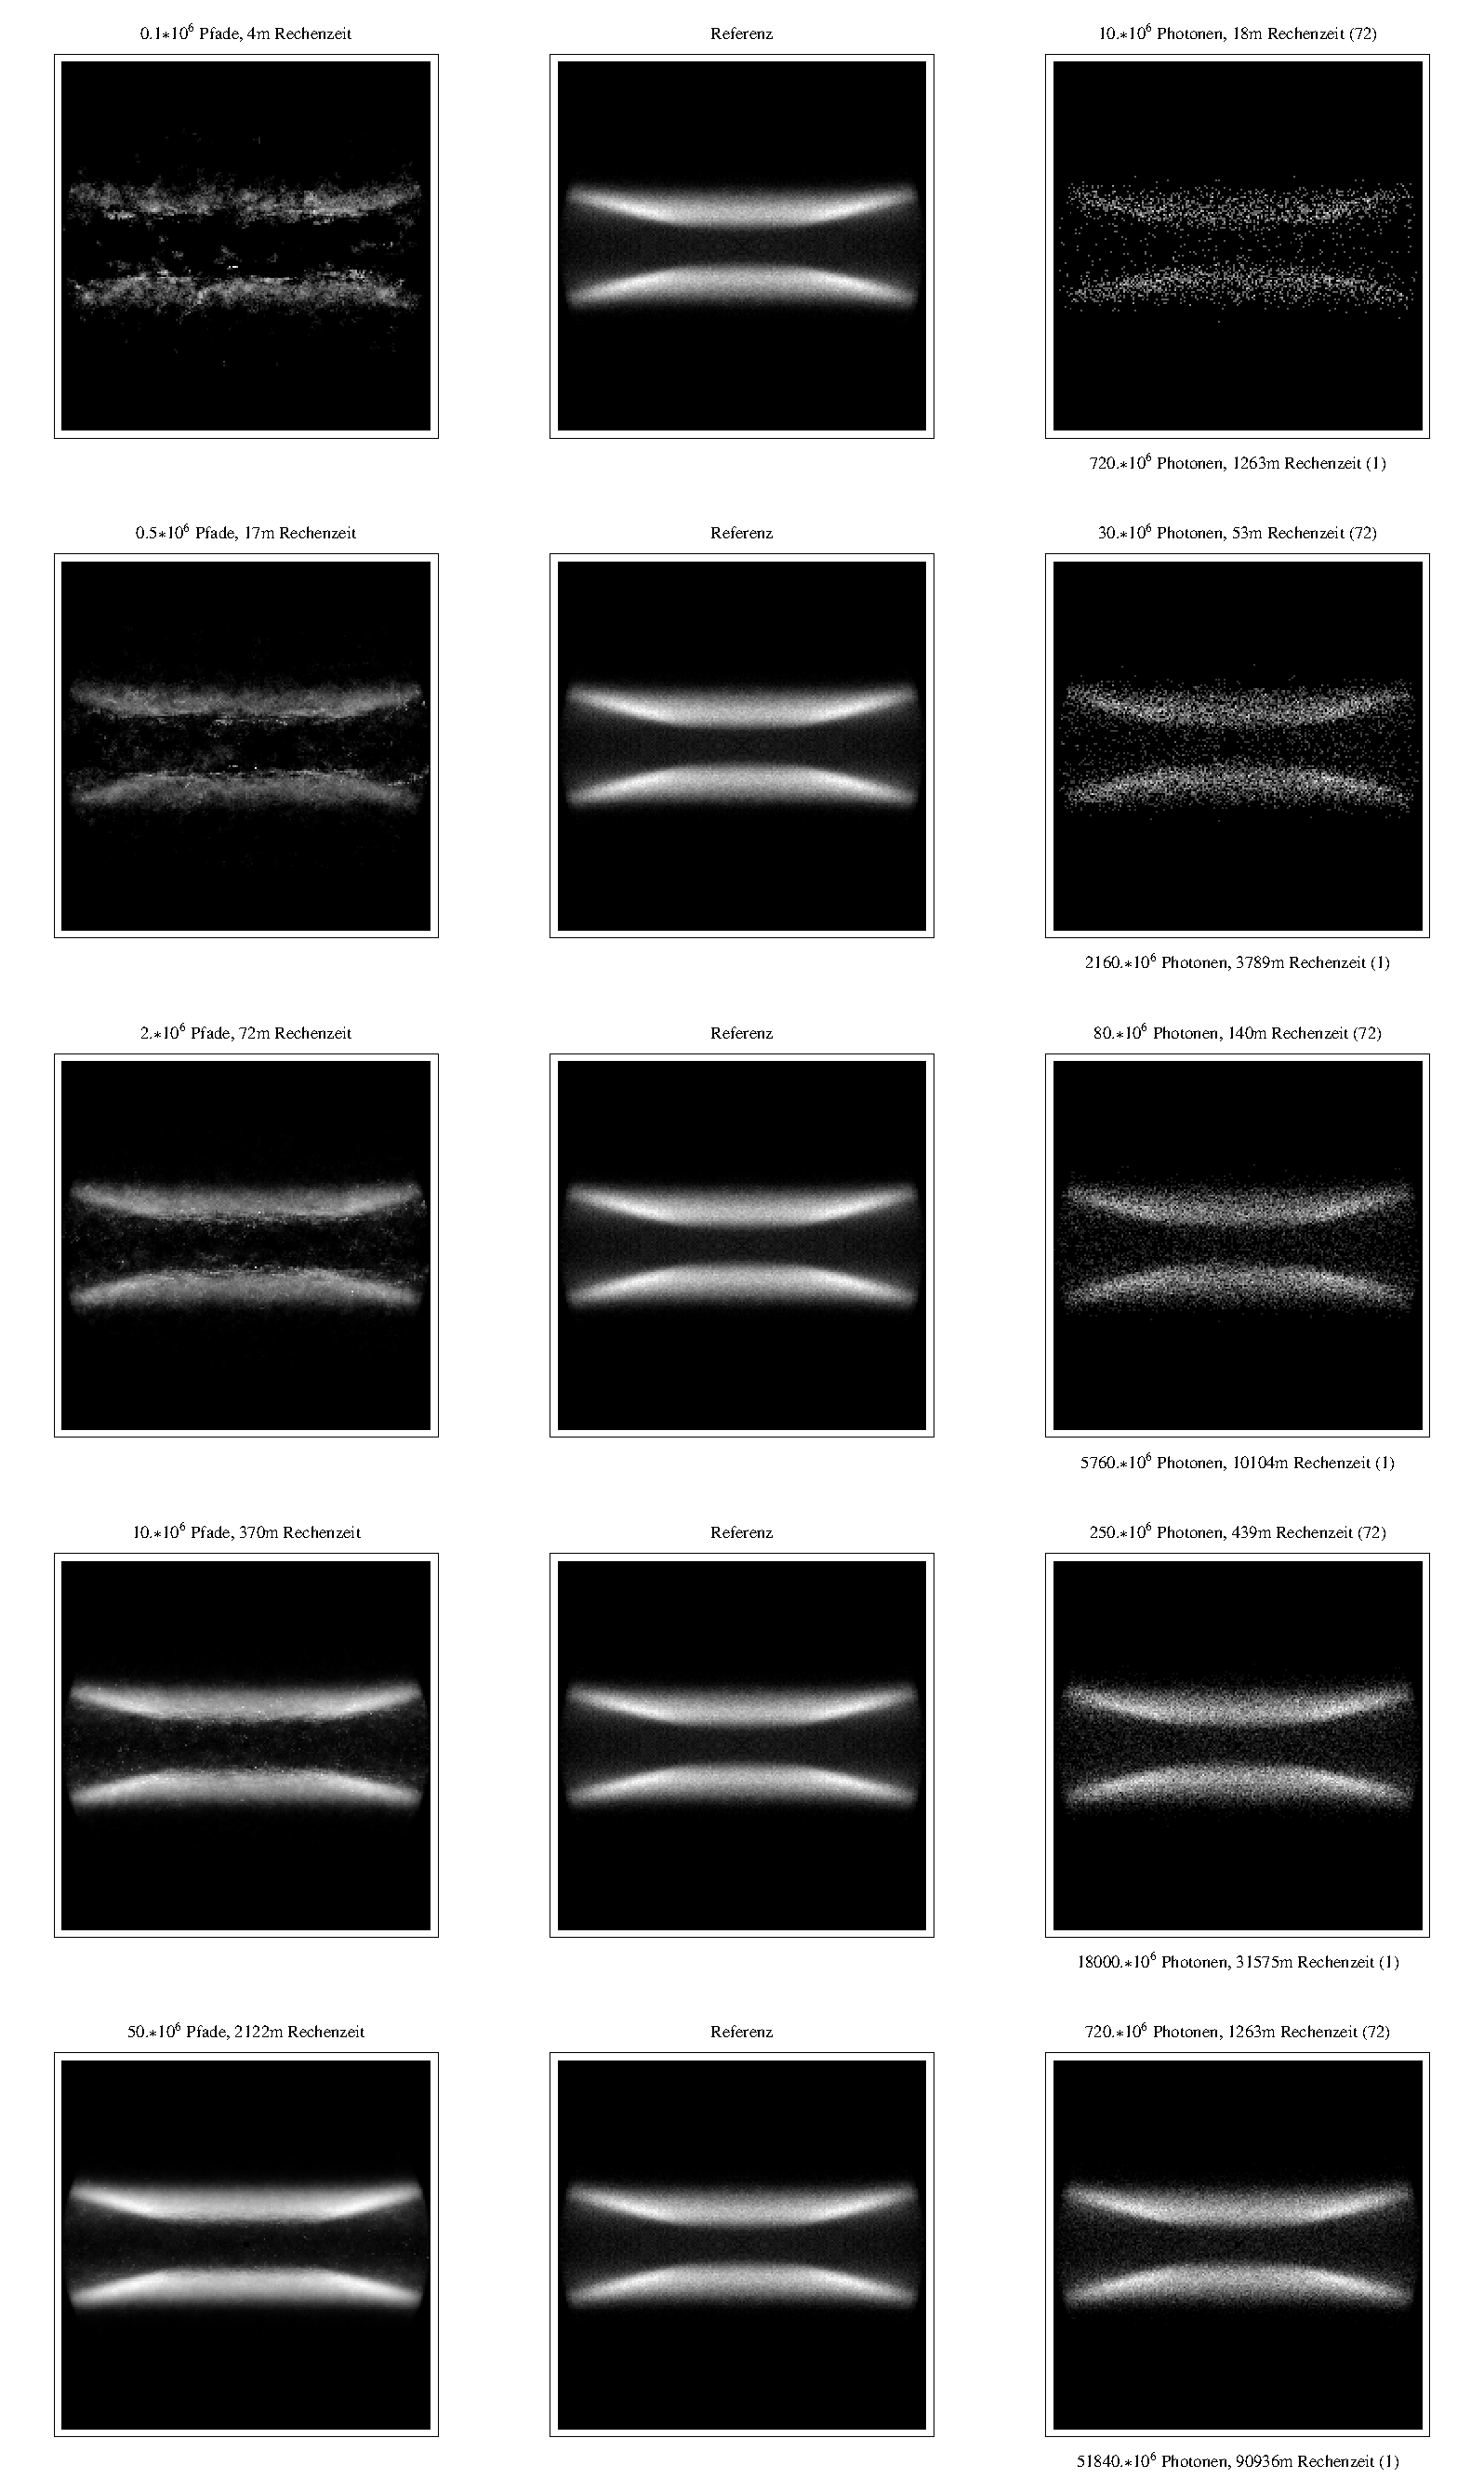
\includegraphics[height=1.0\textheight]{diskimageoverview.eps}
			\caption{übersicht über die Qualität der Bilder bei unterschiedlich langen Simulationsläufen. Bei den \texttt{MC3D}--Bildern in der rechten Spalte repräsentieren die Zahlen in Klammern die Anzahl der benutzten Kameraebenen.}
			\label{fig:disk_image_overview}
		\end{figure}
	
	Wie beim ersten Testfall bestimmen wir auch hier die absoluten Fehler der Streubilder. Als Referenzbild dient die Summe aller 72 Kameraebenen der \texttt{MC3D}--Simulation, die wir noch jeweils horizontal, vertikal und am Ursprung spiegeln und anschließend über die vier Variationen mitteln.

	In Abbildung \ref{fig:disk_contours}	lässt sich erkennen, dass die Ergebnisse qualitativ gut übereinstimmen. Durch erzwungene Streuung und Berücksichtigung nichtangenommener Pfade (siehe Abschnitt \ref{cha:program_description}) reicht der konvergierte Bereich im \texttt{PIRaTE}--Bild weiter nach oben und unten hinaus als im \texttt{MC3D}--Bild.
	
		\begin{figure}
			\centering
			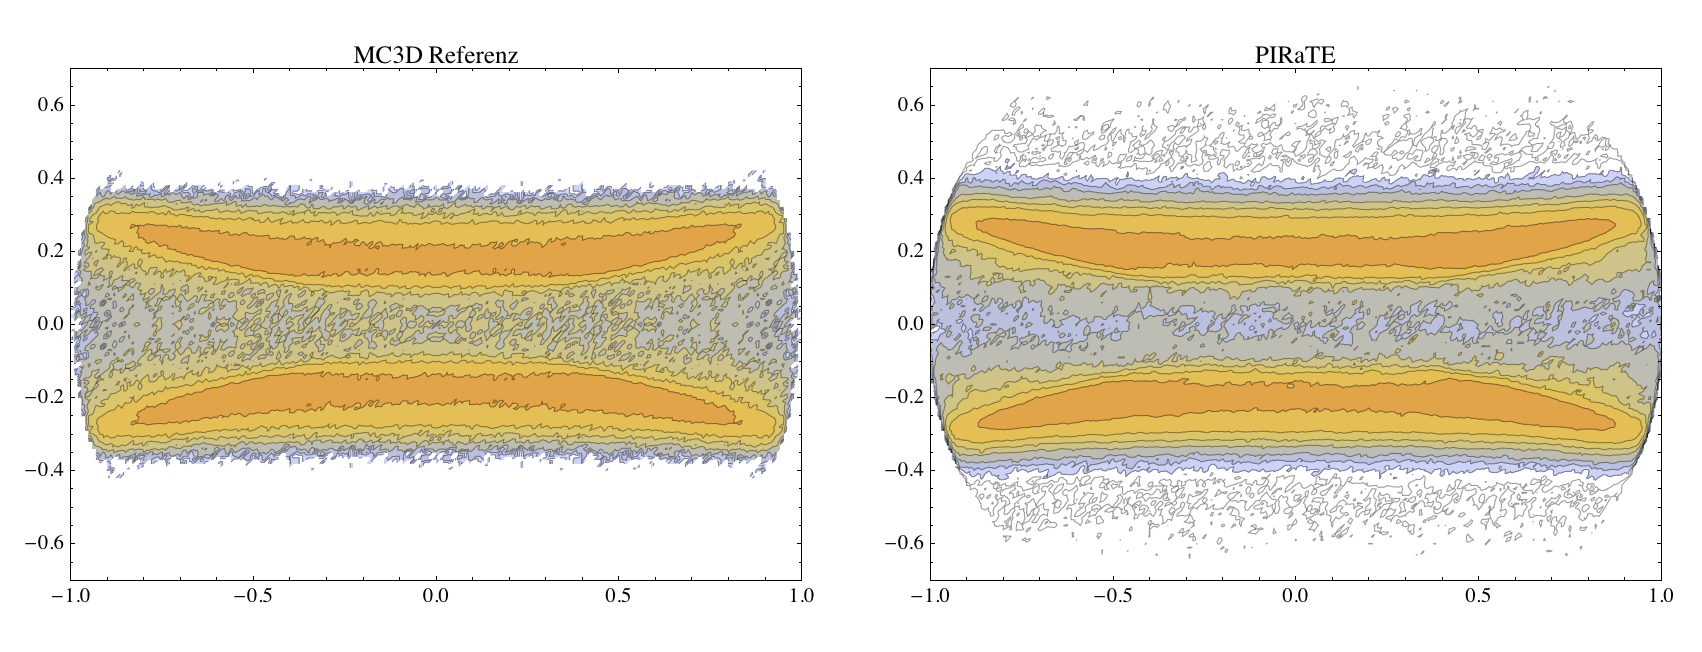
\includegraphics[width=1.0\textwidth]{diskcontourplots.eps}
			\caption{Konturplots des Referenzbildes und des von \pirate generierten Bildes.}
			\label{fig:disk_contours}
		\end{figure}
	
	Schauen wir uns die absoluten Fehler, aufgetragen über die Anzahl generierter Pfade bzw. Photonen, an (siehe Abb.~\ref{fig:disk_error}), schneidet \pirate anfangs vergleichbar gut ab wie \mctd mit 72 Kameraebenen. In Bezug auf die Rechenzeit sogar um eine Größenordnung besser.
	
		\begin{figure}
			\centering
			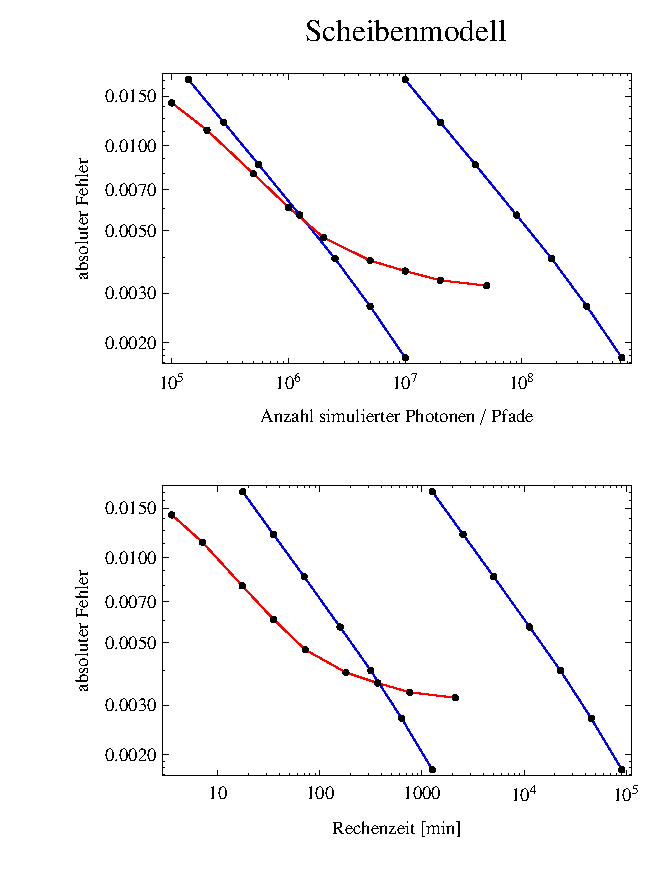
\includegraphics[width=1.0\textwidth]{diskerrorplot.eps}
			\caption{Die rote Linie repräsentiert \pirate--Simulationen. Die blauen Linien repräsentieren \mctd. Die linke Linie steht für Simulationen mit 72, die rechte für Simulationen mit einer Kameraebene.}
			\label{fig:disk_error}
		\end{figure}
	
	Hin zu größeren Pfadanzahlen nähert sich der Fehler allerdings asymptotisch einem Wert größer null, was bedeutet, dass \pirate nicht exakt gegen dasselbe Bild konvergiert. In Abb.~\ref{fig:resdiskplot} ist die Abweichung qualitativ farblich dargestellt. Es ist zu erkenn, dass im Innenbereich das Bild von \pirate zu dunkel ist. Es konnte bisher allerdings nicht geklärt werden, ob die Ursache in einer Abweichung des Modells, einem Programmfehler oder im Verfahren begründet liegt.
	
		\begin{figure}
			\centering
			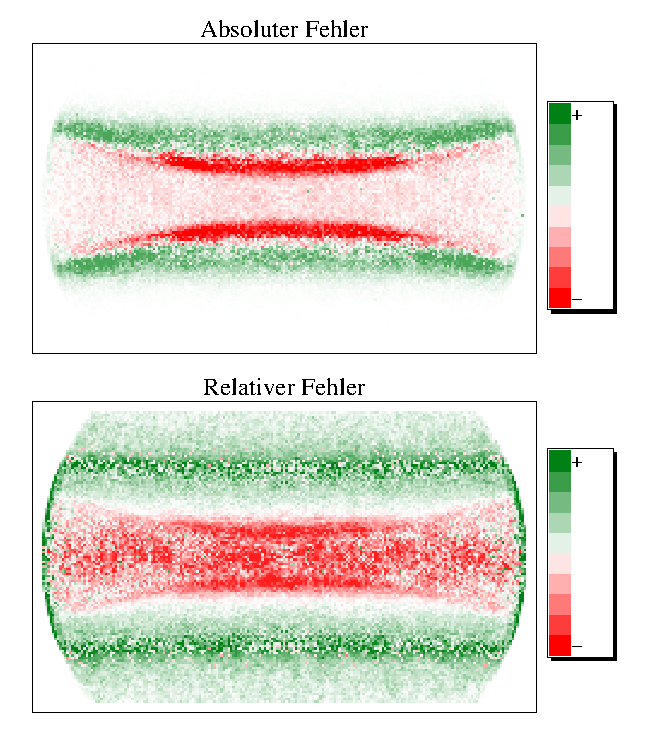
\includegraphics[width=1.0\textwidth]{resdiskplot.eps}
			\caption{Darstellung der Abweichung zwischen dem mit \pirate erzeugten Streubild und dem \texttt{MC3D}--Referenzbild. Rot bedeutet kleinere Werte als im Referenzbild, grün größere.}
			\label{fig:resdiskplot}
		\end{figure}
	

	\section{Einordnung der Resultate}
	Fassen wir die Resultate der beiden Testfälle zusammen, können wir feststellen, dass \pirate für moderate optische Tiefen ($\tau < 10$) häufig eine Größenordnung weniger Pfade braucht, um einen ähnlichen Rauschpegel wie \mctd mit 72 Kameraebenen zu erreichen. Bei kleinen optischen Tiefen ist die Effizienz, bedingt durch erzwungene Streuung und das Zählen nichtangenommener Pfade, sogar noch erheblich größer. In Bezug auf die Rechenzeit ist die Effizienz im Vergleich zu \mctd mindestens ebensogut wie in Bezug auf die Anzahl der Pfade. Dies prädestiniert \pirate insbesondere für irreguläre Dichteverteilungen, bei denen die Verwendung mehrerer Kameraebenen bei der Berechnung eines Bildes aus einem bestimmten Blickwinkel nicht möglich ist. Auf der negativen Seite ist zu erwähnen, dass die momentan implementierte Pfadgenerierungsmethode bei großen, nicht umgehbaren, optischen Tiefen ($\tau>10$) ineffizient wird. Hier wäre es interessant, andere Pfadgenerierungsmethoden, die auf den optisch dicken Fall optimiert sind, zu entwickeln. Ein hierfür vielversprechnender Ansatz findet sich bei \citet{Laszlo:2005p11056}\footnote{siehe hierzu auch \citep{DAldous:1994p11528} und \citep{Grassberger:2002p10876}}. Die Berechnung des direkten Lichtanteils in \pirate ist außerdem noch nicht fehlerfrei. Hier muss genauer geklärt werden, ob es sich um ein Undersamplingproblem, einen falsch definierten Sensor oder um ein anderes Problem handelt. Auch die Abweichungen im inneren Bereich der Scheibe bedürfen einer genaueren Betrachtung und evtl. nötiger Korrekturen. Des Weiteren kann das unnatürlichere Rauschen im Vergleich zu \mctd ein Nachteil sein. Dies läst sich durch Parametertuning der Mutationsstärke verhältnismäßig leicht erreichen.
	
